\documentclass[10pt,a4paper]{article}

\usepackage{commons/course}

\usepackage{listings}
\usepackage{xcolor}


% Define colors for syntax highlighting
\definecolor{keywordstyle}{rgb}{0.0, 0.4, 0.8} % A bluer shade
\definecolor{stringstyle}{rgb}{0.9, 0.17, 0.31} % amaranth
\definecolor{commentstyle}{rgb}{0.1, 0.6, 0.2} % green
\definecolor{numberstyle}{rgb}{0.4, 0.4, 0.4} % gray
\definecolor{backgroundcolor}{rgb}{0.94, 0.97, 1.0} % aliceblue

% Define the Python-like language for syntax highlighting
\lstdefinelanguage{PythonLike}{
	morekeywords={mov, add, sub, cmp, jmp , lw , addi,sw,bne},
	sensitive=false,
	morecomment=[l]{;},
	morestring=[b]",
}

% Set the style for Python-like code
\lstset{
	language=PythonLike,
	basicstyle=\ttfamily\small,
	keywordstyle=\color{keywordstyle},
	stringstyle=\color{stringstyle},
	commentstyle=\color{commentstyle},
	numbers=left,
	numberstyle=\tiny\color{numberstyle},
	stepnumber=1,
	numbersep=5pt,
	keepspaces=true,
	tabsize=4,
	showspaces=false,
	showstringspaces=false,
	showtabs=false,
	breaklines=true,
	breakatwhitespace=false,
	frame=single,
	backgroundcolor=\color{backgroundcolor},
}

\begin{document}
	
	\سربرگ{تمرین سوم}{}{پاسخ‌دهنده: معین آعلی - 401105561}{استاد: سمانه حسینمردی}
	
	
	
	\مسئله{‌}
	\subsection*{الف}
ابتدا همه متغیرهارا مرده فرض کرده و با توجه به الگوریتم، از آخر به عنوان قوانین را چک کرده و ووضعیت متغیرهارا تغییر می‌دهیم:

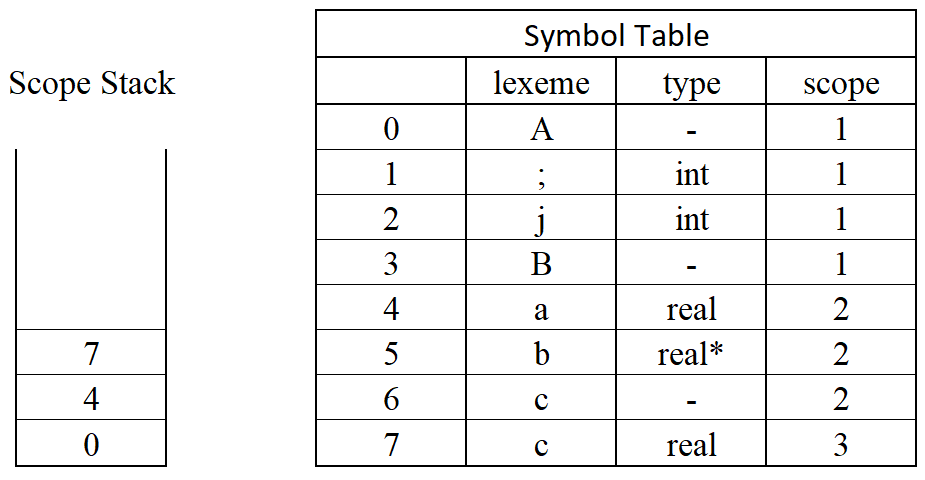
\includegraphics[width=1\linewidth]{figs/1.png}

\pagebreak
\subsection*{ب}
طبق الگوریتم عمل کرده و از اول به آخر جلو رفته و وضعیت متغیرها را تغییر می‌دهیم.

وضعیت اولیه:


\qquad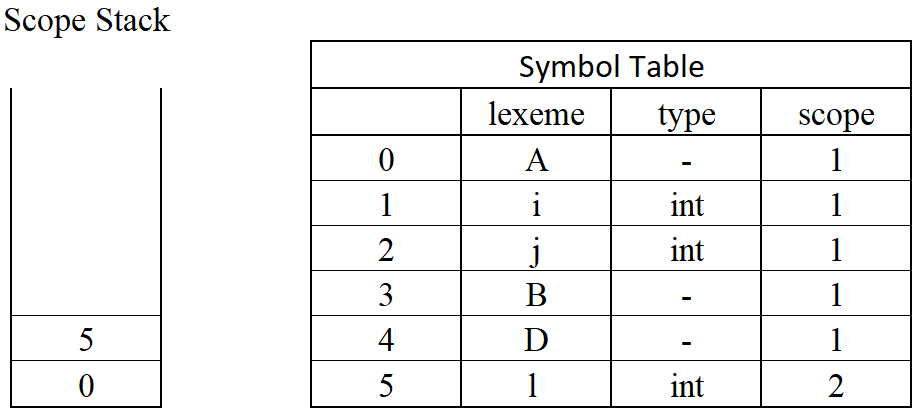
\includegraphics[width=0.8\linewidth]{figs/2.png}


وضعیت نهایی:

\qquad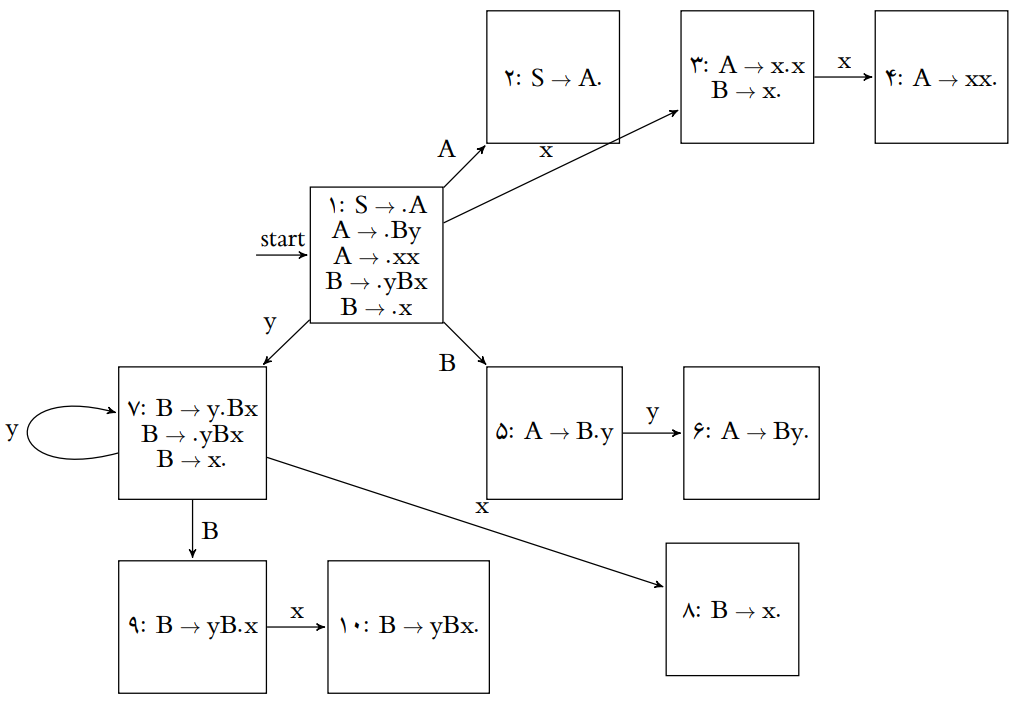
\includegraphics[width=0.8\linewidth]{figs/3.png}














	
	
	
	\مسئله{‌}
	\setLTR
\begin{lstlisting}
program A()
    var i : real
    procedure B(j : integer)
        var k : integer
        i := 0
        j := 6
        k := i + j
    end B
    procedure C(l : integer)
        var l : integer
        procedure D(k : real)
            var a[1..5] : real
            a[j] := 5
            k := 3/i
        end D
    end C
end A
\end{lstlisting}
\setRTL

\subsubsection*{خط 7)} 
\setLTR
$
k:=i+j \xrightarrow{Static \ Error} Type \ Checking \ Error
$
\setRTL
\subsubsection*{خط 10)}
\setLTR
$
var \ l:integer \xrightarrow{Static \ Error} Uniqueness \ Checking \ Error
$
\setRTL
\subsubsection*{خط 13)}
\setLTR
$
a[j]:=5 \xrightarrow{Static \ Error} j \ not \ Defined  \ in \ this \ Scope
$
\setRTL
\subsubsection*{خط 14)}
\setLTR
$
k:=3/i \xrightarrow{Static \ Error} i \ not \ Defined  \ in \ this \ Scope \\ \\
$
\setRTL

تمامی ارورهای این برنامه از نوع Static است و ارور Dynamic ندارد.



	\pagebreak
	
	\مسئله{‌}
	گرامر سوال:
\begin{align*}
	S&\rightarrow Gx \\
	S&\rightarrow yGz \\
	S&\rightarrow Hz \\
	S&\rightarrow yHx \\
	G&\rightarrow w \\
	H&\rightarrow w \\
\end{align*}

ترنزیشن دیاگرم مربوط به گرامر فوق:

\qquad\qquad\qquad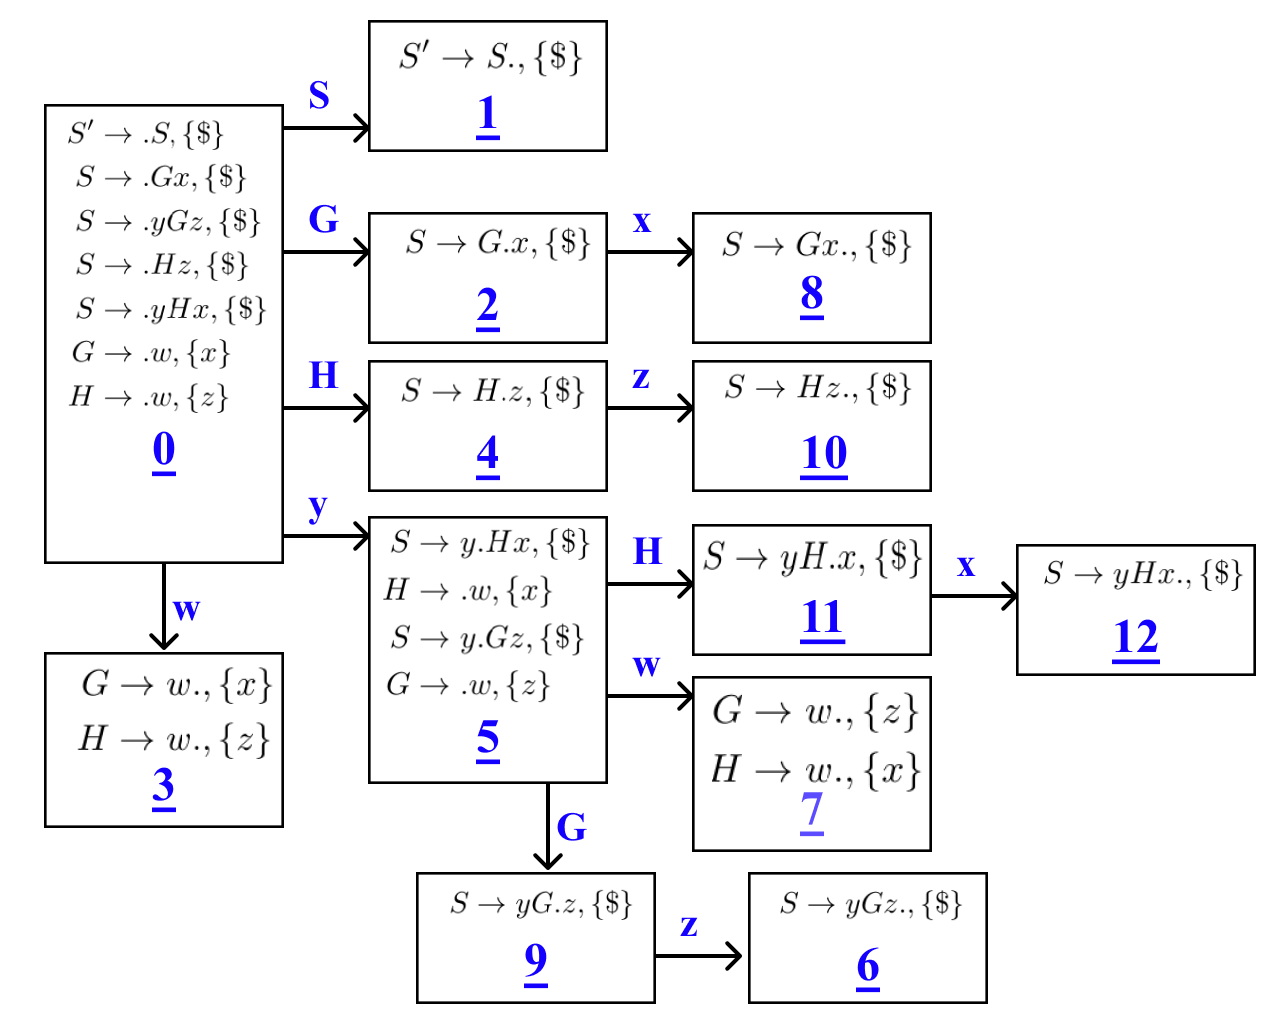
\includegraphics[width=0.7\linewidth]{figs/8.png}

\subsection*{الف}

جدول 
$LR(1)$
مربوط به گرامر فوق:

\qquad\qquad\qquad\qquad\qquad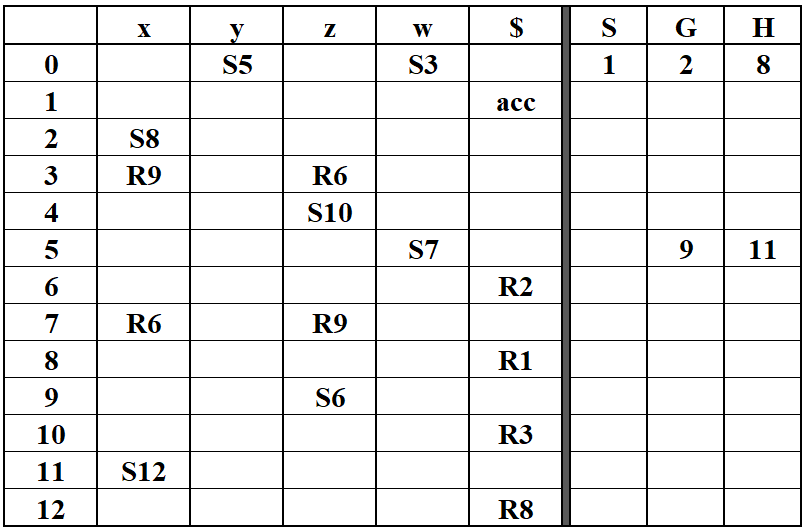
\includegraphics[width=0.5\linewidth]{figs/6.png}
\pagebreak

\subsection*{ب}

جدول 
$LALR(1)$
مربوط به گرامر فوق:

\qquad\qquad\qquad\qquad\qquad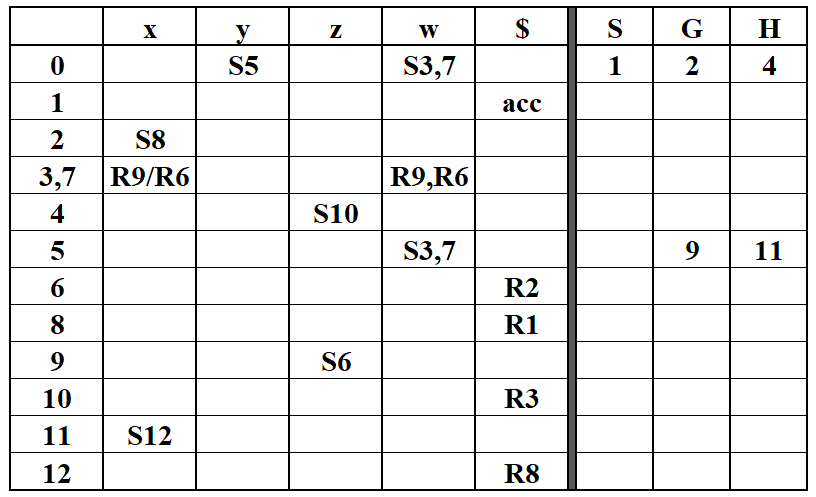
\includegraphics[width=0.5\linewidth]{figs/7.png}

\subsection*{ج}

همانطور که مشخص است، چون جدول 
$LR(1)$
تداخلی ندارد ولی جدول 
$LALR(1)$
دارای تداخل است. پس گرامر فوق از نوع 
$LR(1)$
است.



به عنوان مثال رشته ورودی 
$ywx\$$
را با استفاده از جدول فوق اگر پارس کنیم، داخل خانه 
$(37,x)$
به تداخل می‌خوریم.
















	\pagebreak
	
	\مسئله{‌}
	در ابتدا کد را سه آدرسه مینویسیم:
\setLTR
\begin{lstlisting}
x:=2
y:=3
z:=x+y
x:=4
w:=z*2
\end{lstlisting}
\setRTL
حال مقدار عددی متغیرها را جایگزین کرده:
\setLTR
\begin{lstlisting}
x:=2
y:=3
z:=2+3
x:=4
w:=z*2
\end{lstlisting}
\setRTL
حال عملیات جمع را ساده کرده و ضرب را به شیفت تبدیل میکنیم:
\setLTR
\begin{lstlisting}
x:=2
y:=3
z:=5
x:=4
w:=z<<1
\end{lstlisting}
\setRTL
متغیرهای x و y اضافی هستند، آنها را حذف میکنیم:
\setLTR
\begin{lstlisting}


z:=5

w:=z<<1
\end{lstlisting}
\setRTL
حال مقدار z را جایگزین میکنیم:
\setLTR
\begin{lstlisting}




w:=5<<1
\end{lstlisting}
\setRTL
و در آخر عبارت شیفت را ساده میکنیم:
\setLTR
\begin{lstlisting}




w:=10
\end{lstlisting}
\setRTL
	\pagebreak
	
		\مسئله{‌}
	وضعیت $symbol table$ و $scope stack$ بعد از خط 10 به صورت مقابل است:

\qquad\qquad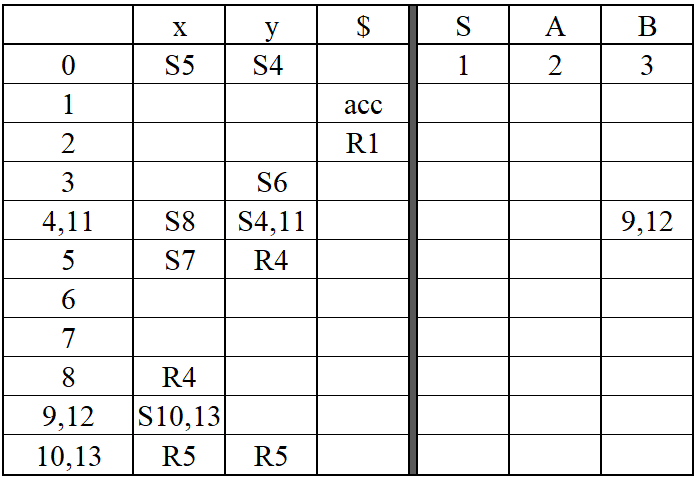
\includegraphics[width=0.6\linewidth]{figs/5.png}

وضعیت $symbol table$ و $scope stack$ بعد از خط 14 به صورت مقابل است:

\qquad\qquad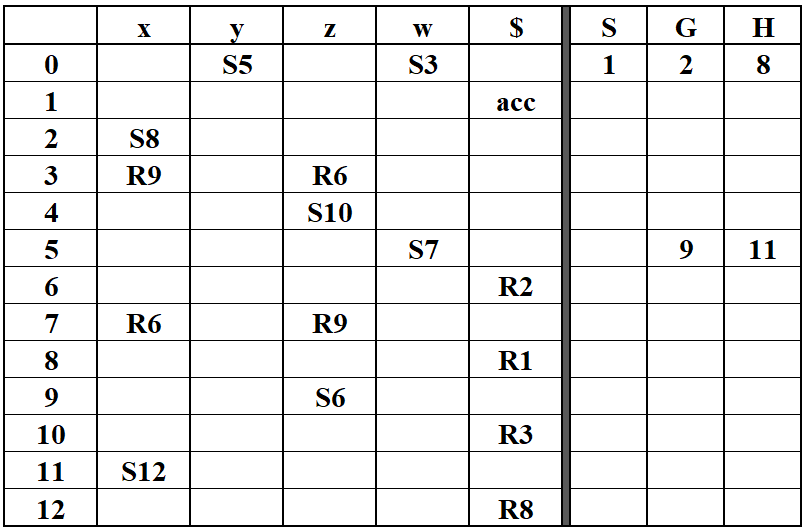
\includegraphics[width=0.6\linewidth]{figs/6.png}
	\pagebreak
	
\end{document}